
\documentclass[runningheads,a4paper,10pt]{etc/llncs}

\usepackage{amssymb}
\usepackage{graphicx}
\usepackage{hyperref}

\usepackage{url}
\usepackage{float}
\usepackage{chngpage}
\usepackage{listings}
\usepackage{apacite}

\usepackage[utf8]{inputenc}
\usepackage[spanish,activeacute]{babel}

\let\stdsection\section
\renewcommand\section{\newpage\stdsection}


\urldef{\mailsa}\path|federico.scenna@gmail.com|    
\newcommand{\keywords}[1]{\par\addvspace\baselineskip
\noindent\keywordname\enspace\ignorespaces#1}
\authorrunning{Federico Scenna}% Part of LEFT running header
\titlerunning{Análisis de grafos del mercado de criptomonedas}% Part of RIGHT running header

\mainmatter  % start of an individual contribution

% first the title is needed
\title{Análisis de grafos del mercado de criptomonedas}

% a short form should be given in case it is too long for the running head

% the name(s) of the author(s) follow(s) next
%
% NB: Chinese authors should write their first names(s) in front of
% their surnames. This ensures that the names appear correctly in
% the running heads and the author index.
%
\author{Federico Scenna\\ [1cm] {\small Tutor: Dr. Ricardo Maronna}}

%

% the affiliations are given next; don't give your e-mail address
% unless you accept that it will be published
\institute{ Maestría en Exploración de Datos y Descubrimiento del Conocimiento \\
Facultad de Ciencias Exactas y Naturales\\ Universidad de Buenos Aires\\
\mailsa
}
\setcounter{tocdepth}{3}


%
% NB: a more complex sample for affiliations and the mapping to the
% corresponding authors can be found in the file "llncs.dem"
% (search for the string "\mainmatter" where a contribution starts).
% "llncs.dem" accompanies the document class "llncs.cls".
%

\begin{document}
\let\oldaddcontentsline\addcontentsline
\def\addcontentsline#1#2#3{}
\maketitle
\def\addcontentsline#1#2#3{\oldaddcontentsline{#1}{#2}{#3}}

\newpage

\paragraph{Resumen} 
En este trabajo se analizan series diarias de precios de distintas criptomonedas entre Agosto del año 2020 y Abril de 2021. A partir de correlaciones de retornos diarios se visualizaron las relaciones entre los distintos activos. Se identificaron mayoritariamente altas correlaciones  entre los movimientos de precios y, durante el periodo analizado, el activo Cardano (ADA) como el activo de referencia del mercado.

\paragraph{Palabras clave} Análisis de grafos, mercados financieros, criptomonedas, blockchain

\tableofcontents

\newpage
\section{Introducción}

Los mercados de criptomonedas adquirieron en los últimos años una gran notoriedad tanto de la prensa como de los agentes de los mercados financieros y sus reguladores. A su vez, se fueron extendiendo sus usos hasta 

\section{Metodología}

\subsection{Fuentes de información y transformación de los datos} 

El objetivo de este trabajo fue analizar los 50 criptoactivos de mayor volumen de mercado del periodo entre 22/8/2020 y 24/4/2021. Se descargaron series de precios del sitio coinmarketcap.com a través de la libreria de R crypto.
https://www.rdocumentation.org/packages/crypto/versions/1.1.3

De esta manera, se obtuvo una lista de activos tanto volátiles como estables (estos últimos fueron diseñados para mantener un valor similar al dólar estadounidense). Se estableció el dato de que tipo de activo era cada uno así se podía identificar en el grafo.

Previamente a la construcción del grafo, era necesario establecer alguna métrica para desestacionalizar la serie de precios de los activos para evitar correlaciones espurias. Uno de los métodos más frecuentes que propone la literatura es la tasa de retorno logarítmica: 


$log=\frac{log(price_t)}{log(price_{t-1})}$


Se decidió, a modo de mantener la claridad en el análisis y por las cualidades propias del este tipo de mercado, computar retornos diarios de cada uno de los activos. 
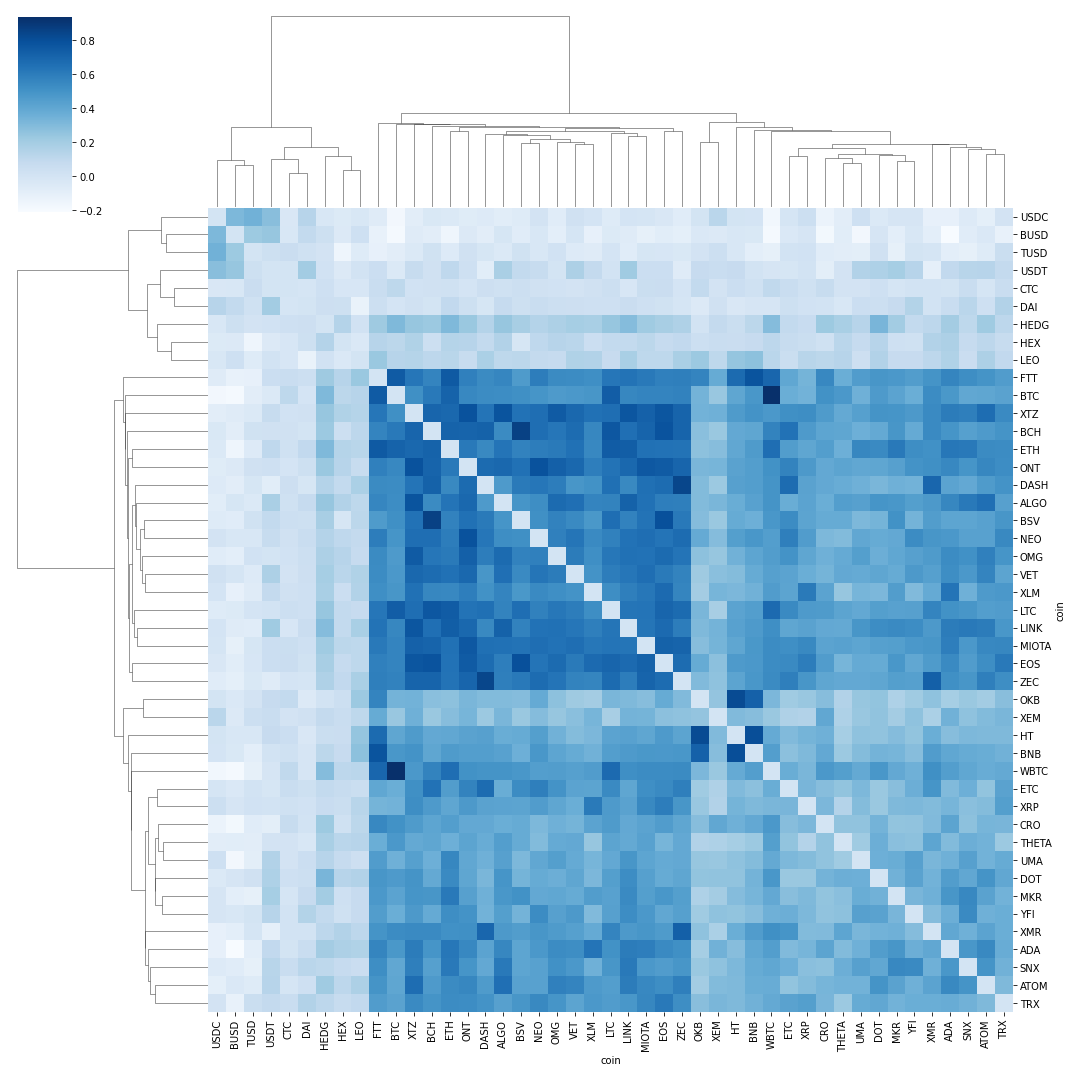
\includegraphics[scale=.35]{images/corr_matrix.png}

\subsection{Construcción de grafos}

En la literatura, la metodología usualmente propuesta es la creación de un grafo a partir de una matriz de correlación a partir de un punto de corte determinado. En base a la distrubición de la correlación y a la intermediación promedio de la red.

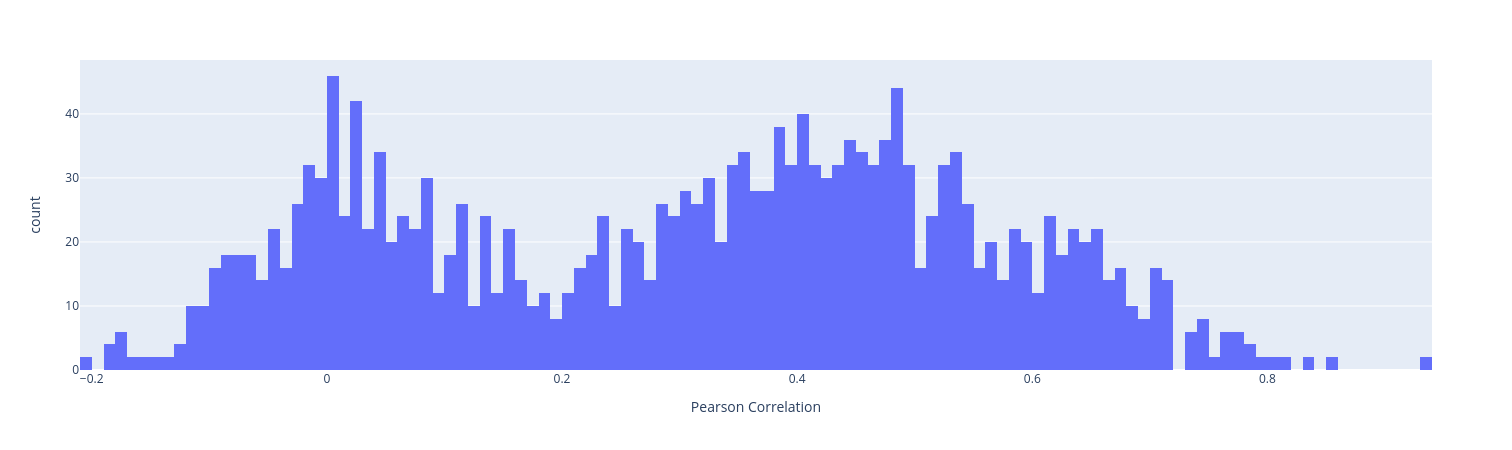
\includegraphics[scale=.35]{images/correlation_hist.png}

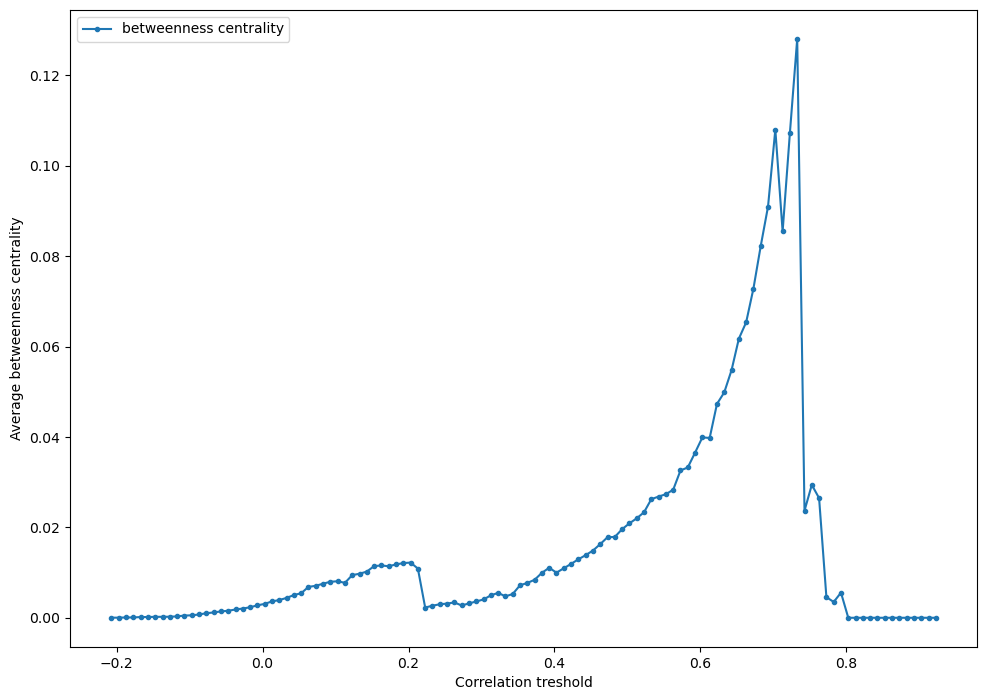
\includegraphics[scale=.35]{images/betweeness_centrality.png}


\subsection{Distribución de nodos}


\section{Comunidades}

\section{Conclusiones}

\bibliographystyle{apacite}
\bibliography{citations}

\end{document}